\documentclass[10pt,leter,openany]{article}
\usepackage[utf8]{inputenc}
\usepackage[english]{babel}
\usepackage{amsmath}
\usepackage{amsfonts}
\usepackage{amssymb}
\usepackage{graphicx}
\usepackage{listings}
\usepackage{color}
\usepackage[left=3cm,right=3cm,top=3cm,bottom=3cm]{geometry}
\usepackage[numbers,sort&compress]{natbib}
\usepackage{url}
\usepackage{caption}
\usepackage{siunitx}
%\usepackage{subfigure}
\usepackage{float}
\usepackage{booktabs}
\usepackage{subcaption}
\usepackage{comment}
\usepackage{mwe}
%\usepackage[table,xcdraw]{xcolor}
\usepackage[shortlabels]{enumitem}   %To enumerate with letters
\usepackage{mathtools}	%To write derivates
\usepackage[thinc]{esdiff}	%To write derivates
\usepackage{cancel} %To cancel terms in equations

\setlength{\parindent}{0pt}
\setlength{\parskip}{4pt}

\definecolor{mygreen}{rgb}{0,0.6,0}
\definecolor{mygray}{rgb}{0.5,0.5,0.5}
\definecolor{mymauve}{rgb}{0.58,0,0.82}

\lstset{ 
	backgroundcolor=\color{white},   % choose the background color; you must add \usepackage{color} or \usepackage{xcolor}; should come as last argument
	basicstyle=\footnotesize,        % the size of the fonts that are used for the code
	breakatwhitespace=false,         % sets if automatic breaks should only happen at whitespace
	breaklines=true,                 % sets automatic line breaking
	captionpos=b,                    % sets the caption-position to bottom
	commentstyle=\color{mygreen},    % comment style
	deletekeywords={...},            % if you want to delete keywords from the given language
	escapeinside={\%*}{*)},          % if you want to add LaTeX within your code
	extendedchars=true,              % lets you use non-ASCII characters; for 8-bits encodings only, does not work with UTF-8
	firstnumber=01,                	 % start line enumeration with line 1000
	frame=single,	                 % adds a frame around the code
	keepspaces=true,                 % keeps spaces in text, useful for keeping indentation of code (possibly needs columns=flexible)
	keywordstyle=\color{blue},       % keyword style
	language=Python,                 % the language of the code
	morekeywords={*,...},            % if you want to add more keywords to the set
	numbers=left,                    % where to put the line-numbers; possible values are (none, left, right)
	numbersep=5pt,                   % how far the line-numbers are from the code
	numberstyle=\tiny\color{mygray}, % the style that is used for the line-numbers
	rulecolor=\color{black},         % if not set, the frame-color may be changed on line-breaks within not-black text (e.g. comments (green here))
	showspaces=false,                % show spaces everywhere adding particular underscores; it overrides 'showstringspaces'
	showstringspaces=false,          % underline spaces within strings only
	showtabs=false,                  % show tabs within strings adding particular underscores
	stepnumber=1,                    % the step between two line-numbers. If it's 1, each line will be numbered
	stringstyle=\color{mymauve},     % string literal style
	tabsize=2,	                     % sets default tabsize to 2 spaces
	title=\lstname                   % show the filename of files included with \lstinputlisting; also try caption instead of title
}

\usepackage[dvipsnames,table,xcdraw]{xcolor}

\usepackage{fancyvrb}

% redefine \VerbatimInput
\RecustomVerbatimCommand{\VerbatimInput}{VerbatimInput}%
{fontsize=\footnotesize,
	%
	frame=lines,  % top and bottom rule only
	framesep=2em, % separation between frame and text
	rulecolor=\color{Gray},
	%
	label=\fbox{\color{Black}data.txt},
	labelposition=topline,
	%
	commandchars=\|\(\), % escape character and argument delimiters for
	% commands within the verbatim
	commentchar=*        % comment character
}



\usepackage{titling}
\newcommand{\subtitle}[1]{%
	\posttitle{%
		\par\end{center}
	\begin{center}\large#1\end{center}
	\vskip0.5em}%
}


\author{5273}
\title{Homework Assignment 14: Applied Probabilistic Models}
\subtitle{Central Limit Theorem}
\date{}


\begin{document}
	
\maketitle

\section{Introduction}

	Central Limit Theorem (CLT) is an approximation one can use when the population to study is quite big (it would take a long time to gather data about each individual) and identifying its characteristics is desired. In statistical terms, one collects samples from a population and by combining the information from the samples, conclusions can be drawn about the population. In a nutshell, the approach of the CLT could be:
\begin{itemize}
	\item Draw multiple samples sufficient in size.
	\item Calculate the individual mean of these samples.
	\item Calculate the mean of these sample means, and this value will give the approximate mean of the studied variable.
	\item Additionally, the histogram of the sample means will resemble a bell curve or normal distribution.
\end{itemize}

\section{Applications}

	In this section, it is seen how the CLT can be used in real-world problems and how to apply it. It helps to solve problems where the population is not normal.
	
	\subsection{Manufacturing}

		Let assume a pipe manufacturing organization produces a different kind of pipes and the monthly data of the wall thickness of certain types of pipes are given. The organization wants to analyze the data by constructing confidence intervals to implement some strategies in the future and the challenge is that the distribution of the data is not normal. Data is simulated in R software \citep{r}. Figure \ref{fig:hist_data} shows a histogram of all the observations of the data. This graph denotes with a vertical red line the population mean, which is 12.802 and one can see that the population is not normal.
		
		\begin{figure}
			\begin{center}
				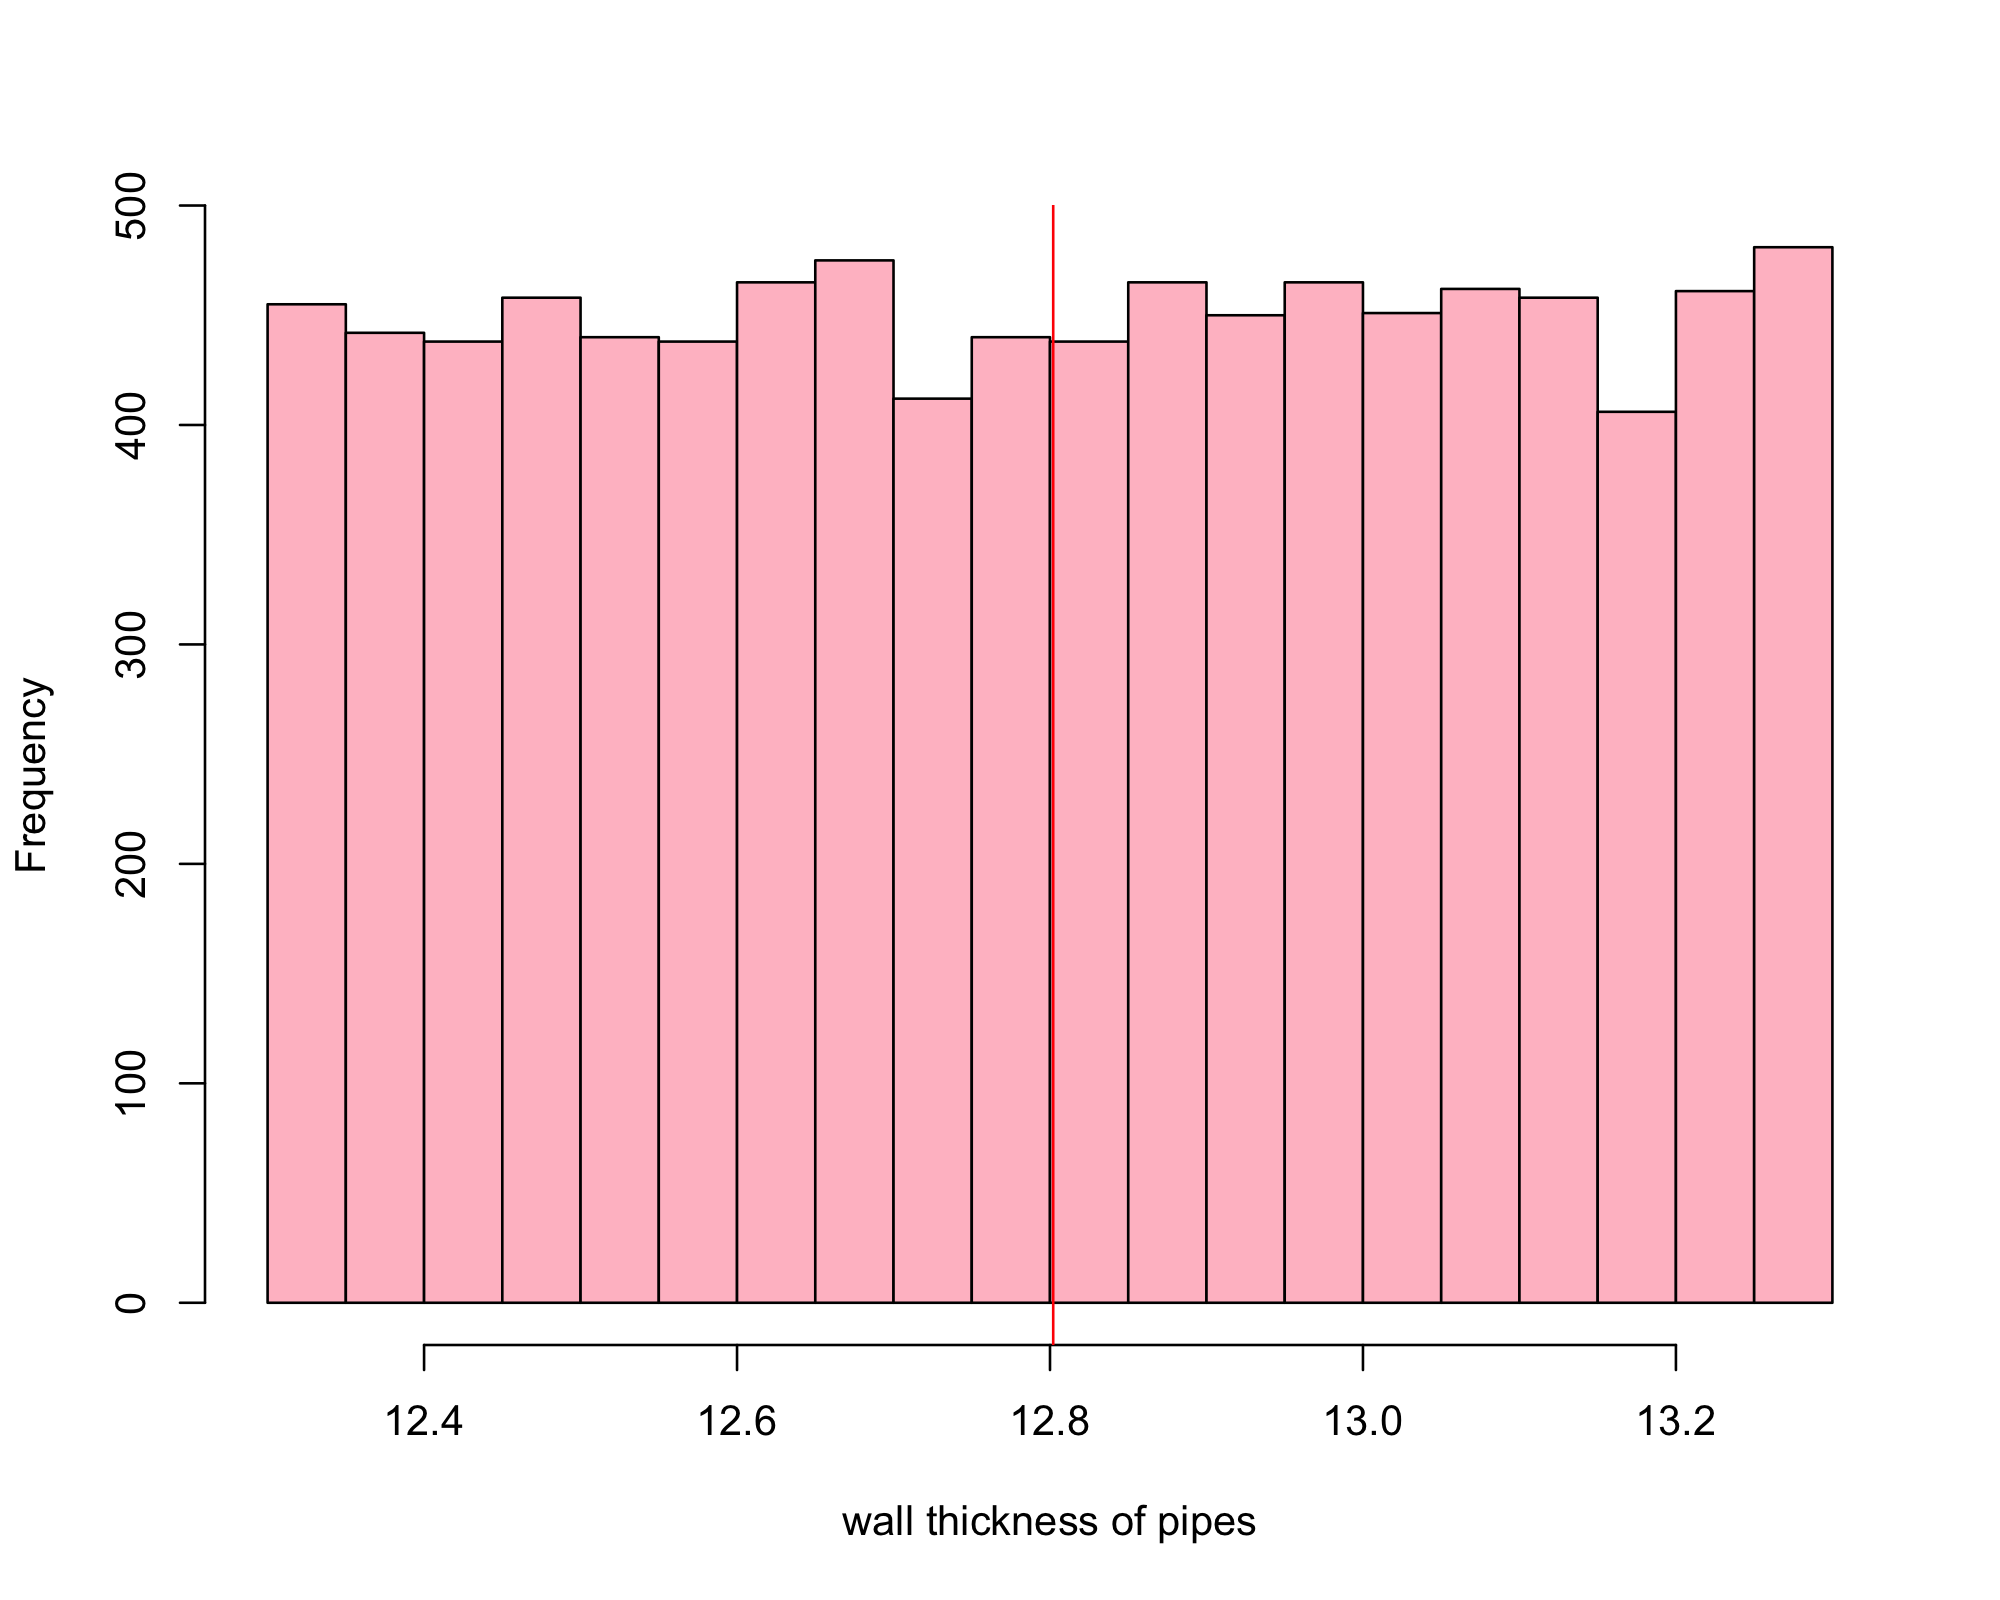
\includegraphics[scale=0.15]{img/hist_data}
				\captionof{figure}{Histogram for Wall Thickness }
				\label{fig:hist_data}
			\end{center}
		\end{figure}
		
		Therefore, to apply the CLT, it is needed to draw sufficient samples of different sizes and compute their means (known as sample means). Figure \ref{fig:hist_sample_means} shows this experiment, where sufficient samples are drawn, increasing its sizes. Means are calculated and are plotted in R. It is known that the minimum sample size taken should be 30, but even with samples of size 10, (see Figure \ref{fig:sample10}) nice bell-shaped curves are evidenced. The sampling distribution should approach a normal distribution as the sample sizes increase. Therefore, one can consider the sampling distributions as normal and the pipe manufacturing organization can use these distributions for further analysis.
		
			\begin{figure}
				\centering
				\begin{subfigure}[b]{0.45\textwidth}
					\centering
					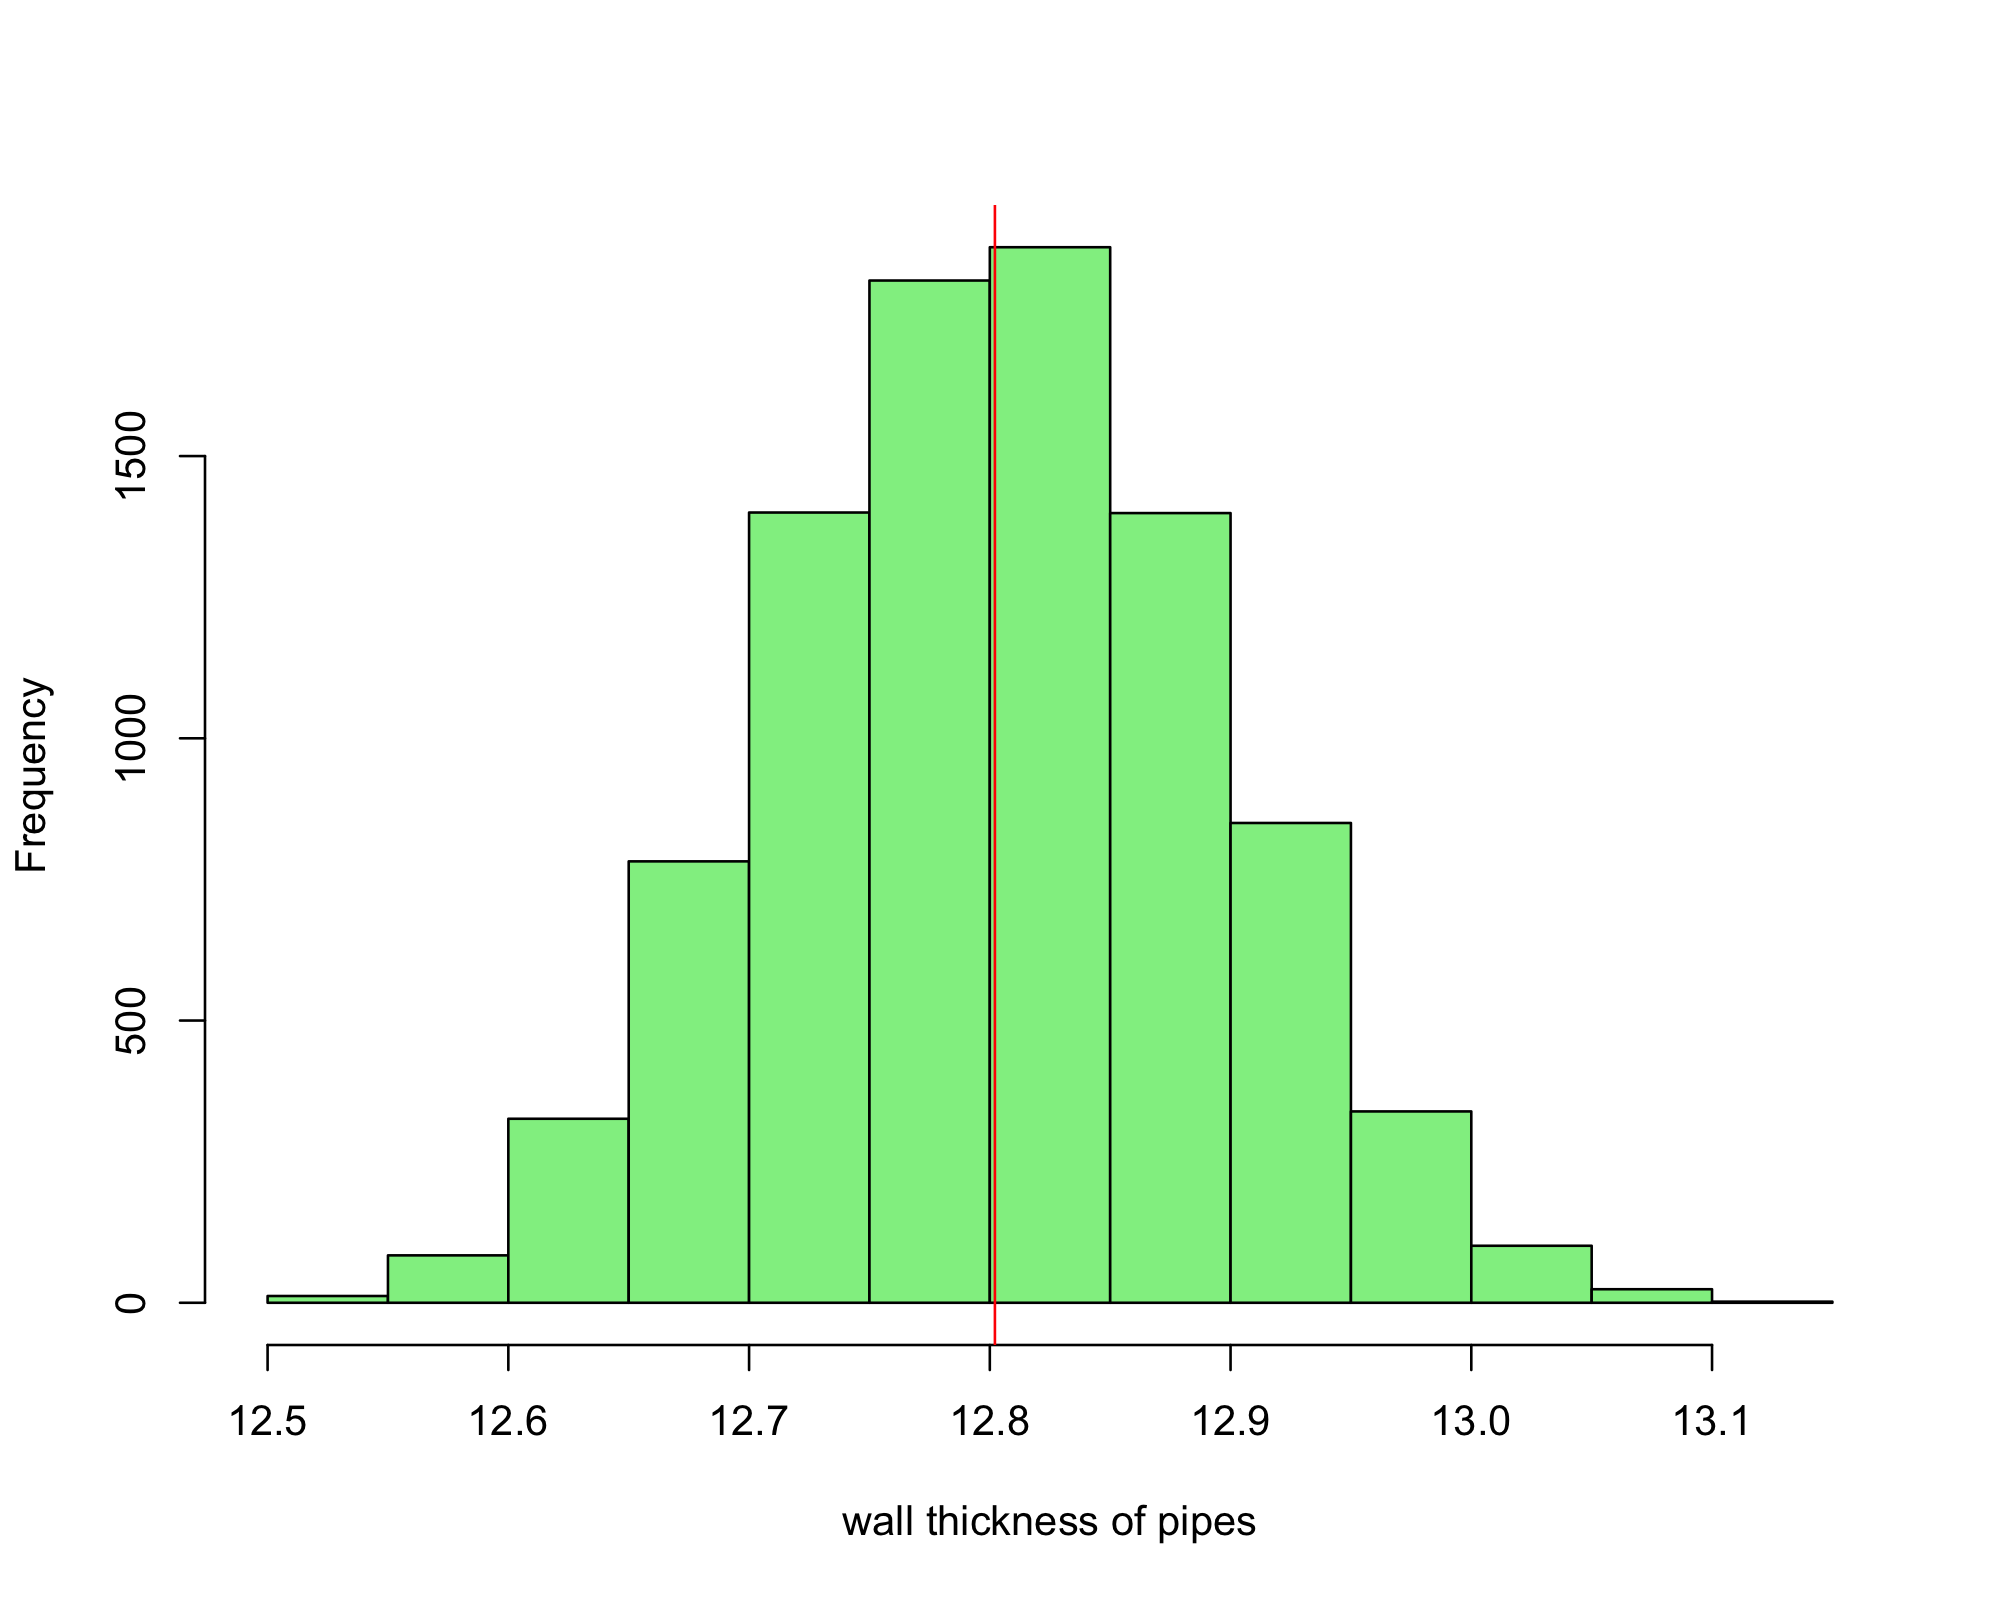
\includegraphics[width=\textwidth]{img/hist_sample10}
					\caption[]%
					{{\small Histogram of samples of size 10}}    
					\label{fig:sample10}
				\end{subfigure}
				\hfill
				\begin{subfigure}[b]{0.45\textwidth}  
					\centering 
					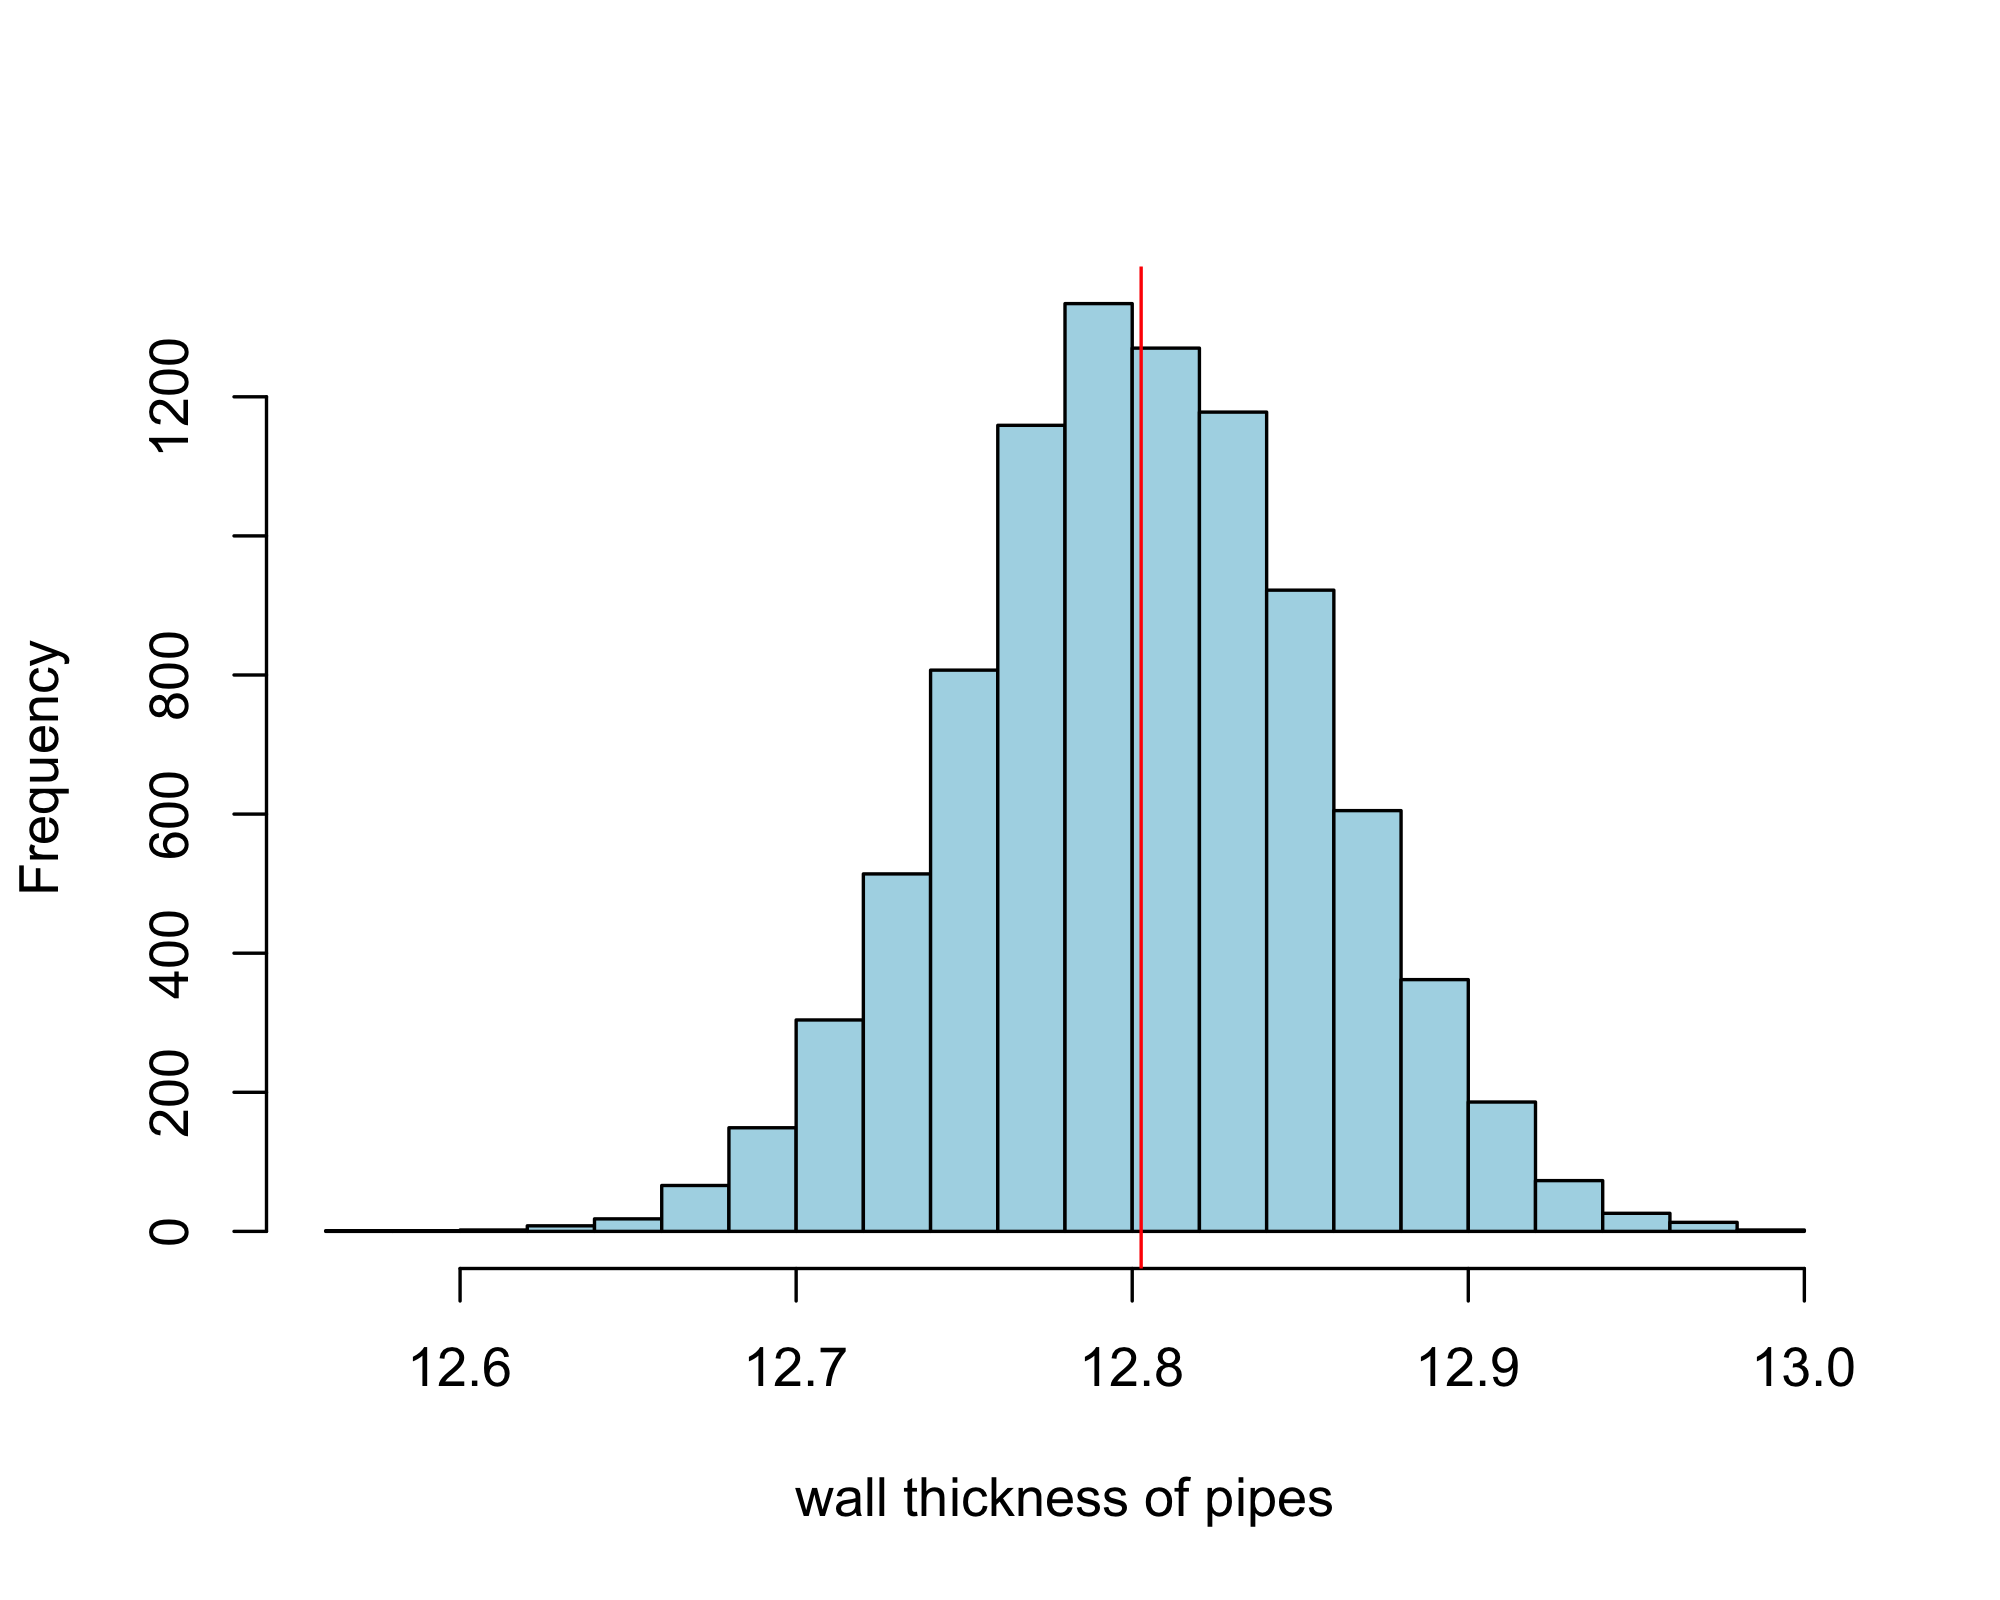
\includegraphics[width=\textwidth]{img/hist_sample30}
					\caption[]%
					{{\small Histogram of samples of size 30}}    
					\label{fig:sample30}
				\end{subfigure}
				\vskip\baselineskip
				\begin{subfigure}[b]{0.45\textwidth}   
					\centering 
					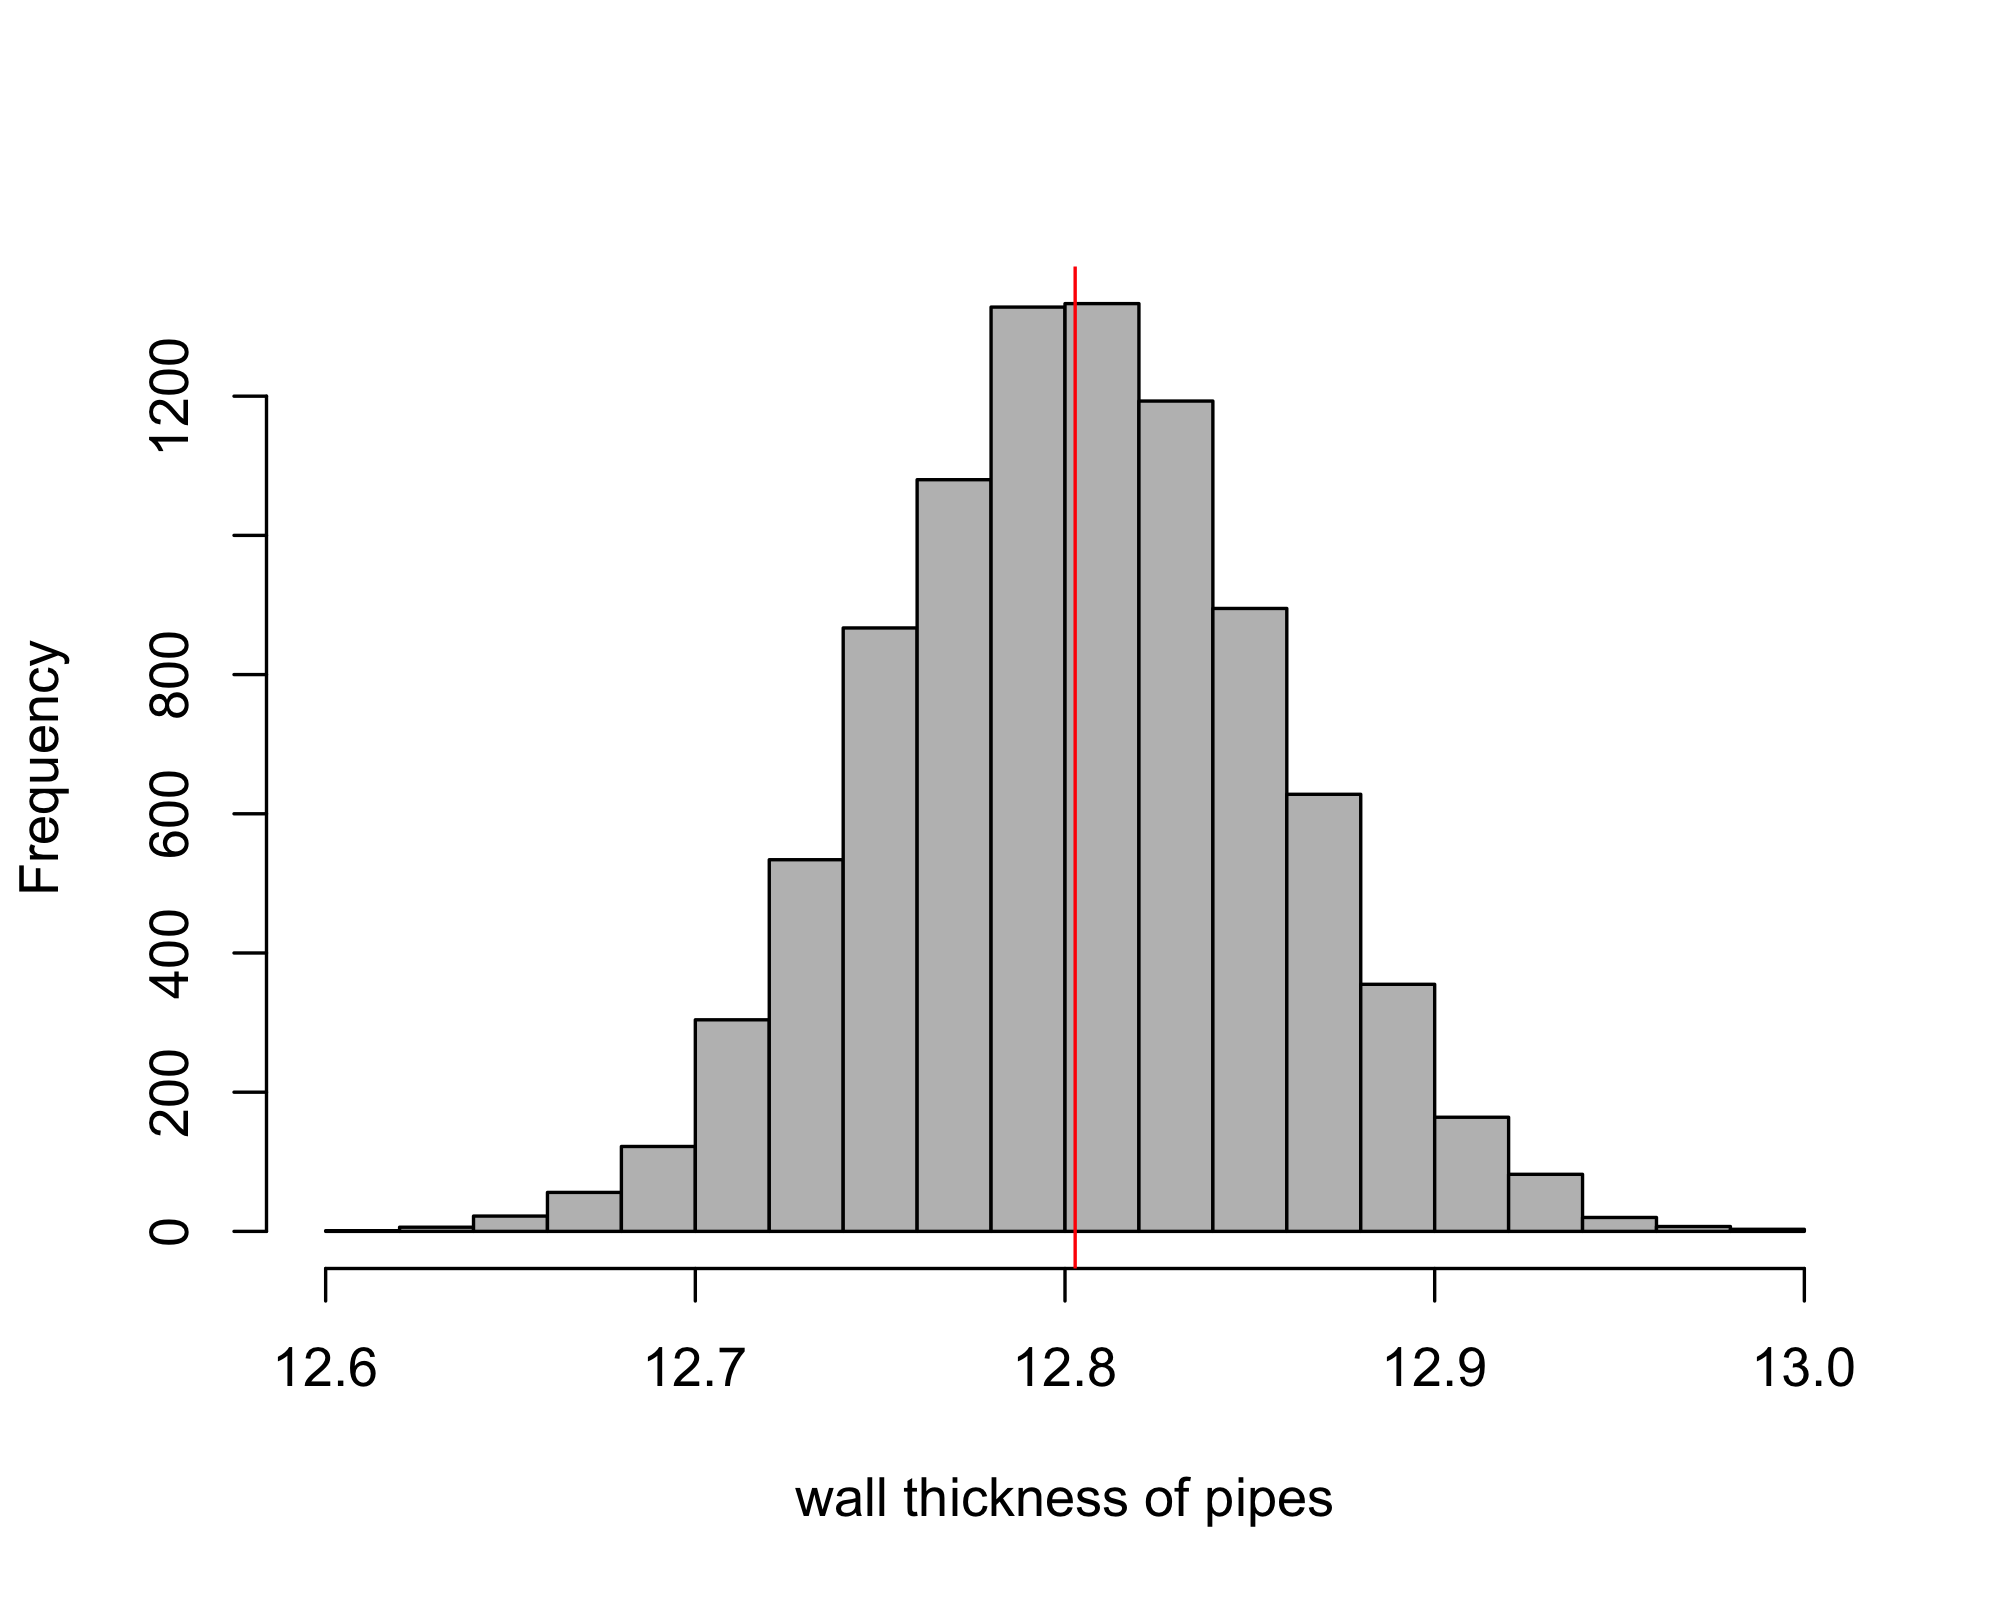
\includegraphics[width=\textwidth]{img/hist_sample50}
					\caption[]%
					{{\small Histogram of samples of size 50}}    
					\label{fig:sample50}
				\end{subfigure}
				\begin{subfigure}[b]{0.45\textwidth}   
					\centering 
					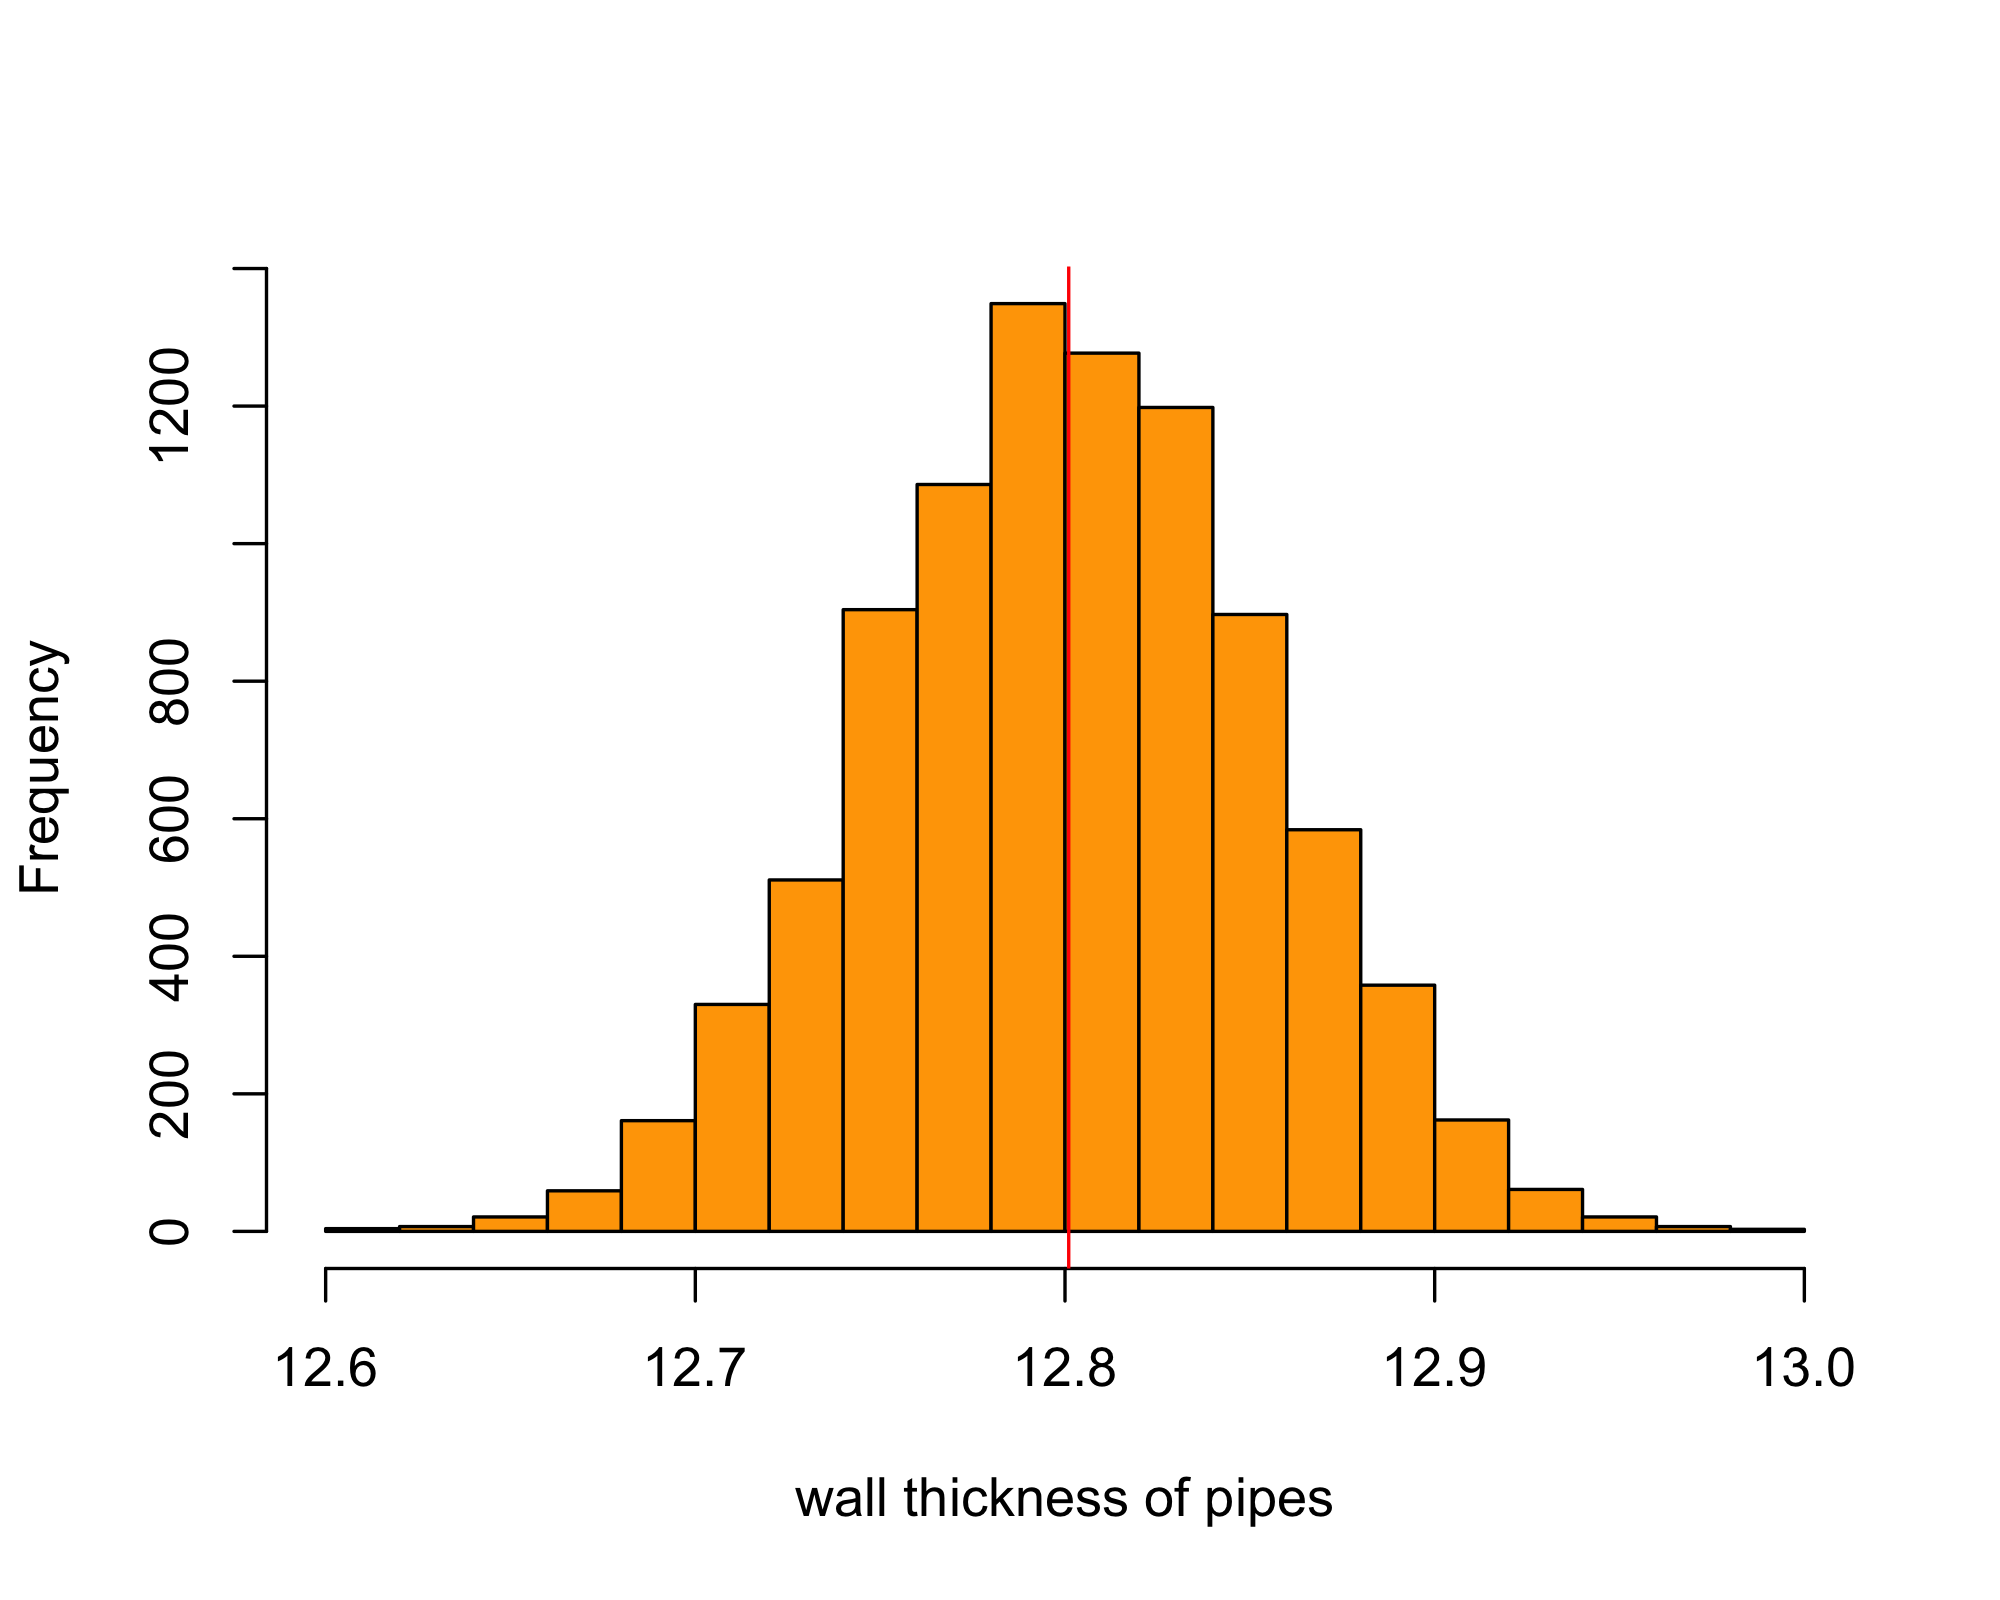
\includegraphics[width=\textwidth]{img/hist_sample500}
					\caption[]%
					{{\small Histogram of samples of size 500}}
					\label{fig:sample500}
			  	\end{subfigure}
				\caption[ ]
				{\small Histograms of the sample means} 
				\label{fig:hist_sample_means}
			\end{figure}
		
		\subsection{Baseball}
		
		Another application can be found by \citet{anderson2014central}, where CLT found an interesting application as hypothesis testing. This author answers the following question using the CLT: \textit{Is there such thing as home-field advantage in Major League Baseball?}
		
		Concerning this problem, the null hypothesis and the alternative hypothesis are: \begin{equation*}
				\begin{aligned}
					H_{0}\mbox{: }& \mbox{There is no home-field advantage},\\
					H_{1}\mbox{: }& \mbox{There is a home-field advantage}.
				\end{aligned}
			\end{equation*}
		
		To test this notion, in a Major League Baseball (MLB) season 2431 games are played. Let us take the 2013 MLB season, were 1308 of those games were won at home, therefore the observed value $\hat{p}=0.5381$. To test the hypothesis, our null hypothesis will be 0.5, that is 50\% of the MLB games are won at home and the other half on the road, hence, there is no home-field advantage. One method is using a confidence interval. For testing, \begin{equation*}
			\begin{aligned}
				H_{0}\mbox{: }& p=0.50,\\
				H_{1}\mbox{: }& p>0.50.
			\end{aligned}
		\end{equation*} at the 0.05 level of significance a right-sided 95\% confidence interval for $p$ can be constructed. If our test statistic of $ p=0.5 $ is in the interval, then we fail to reject $H_{0}$ at the 0.05 level of significance. If $p=0.5$ is not in the interval, we reject $H_{0}$. The right-sided $100(1-\alpha)\%$ confidence interval for $p$ for a large sample is given by \begin{equation*}
			\hat{p} - z_{\alpha} \sqrt{\dfrac{\hat{p}(1-\hat{p})}{n}} < p \leq 1\\,
		\end{equation*} where $\alpha$ is the level of significance.
	
		Since $n=2431, \hat{p} = 0.5381, \alpha = 0.05$, and $z_{0.05} = 1.645$, obtained from the standard normal table \citep{rohlf1995statistical}, which is used to find the probability that a statistic is observed below, above, or between values on the standard normal distribution, and by extension, any normal distribution. Therefore a right-sided 95\% confidence inerval for $p$ is: \begin{equation*}
			\begin{aligned}
			0.5381 - 1.645 \sqrt{\dfrac{(0.5381)(1-0.5381)}{2431}} < p \leq 1,\\
			0.5381 - 1.645(0.0101114)  < p \leq 1,\\
			0.5215 < p \leq 1.
			\end{aligned}
		\end{equation*}
	Since $ 0.5 \notin \left(0.5215,1\right]$, reject $H_{0}: p = 0.5$ in favor of $H_{1}: p > 0.5$ at the 0.05 level of significance, that is, there is enough evidence to support that there is a home-field advantage, and the home team wins more than 50\% of the games played at home, hence there is such thing as home-field advantage in MLB. 
	
	Also, if one wants to see if there is a difference between the American League and the National League a similar analysis can be performed. For these separate leagues, a 99\% confidence interval is used, and for the National League it is obtained that 0.5 $\notin \left(0.5117,1\right] $, therefore it is concluded that the National League has a home-field advantage. On the other hand, in the American League $0.50 \in \left(0.4978,1\right] $, fail to reject $H_{0}: p = 0.50$. That is, one does not have enough evidence to support that there is a home-field advantage in the American League based on the 2013 season.
			
\clearpage

	\bibliography{as14}
	\bibliographystyle{plainnat}
	
\end{document}